\documentclass[10pt]{article}

\usepackage[spanish,mexico]{babel}
\usepackage[utf8]{inputenc}
\usepackage{apacite}

\usepackage{anysize}
\marginsize{2cm}{2cm}{2cm}{2cm}
\setlength{\parskip}{8px}

\usepackage{hyperref}

\usepackage{amsmath}
\usepackage{amssymb}
\usepackage{amsfonts}
\usepackage{cancel}

\usepackage{graphicx}
\usepackage{float}

\usepackage{caption}
\usepackage{subcaption}

\usepackage{xcolor}

\usepackage{fancyhdr}

\usepackage{listings}

\usepackage{longtable}
\usepackage{colortbl}
\usepackage{diagbox}
\usepackage{tabularx}

\usepackage{tcolorbox}


\newcolumntype{L}[1]{>{\hsize=#1\hsize\raggedright\arraybackslash}X}%
\newcolumntype{R}[1]{>{\hsize=#1\hsize\raggedleft\arraybackslash}X}%
\newcolumntype{C}[2]{>{\hsize=#1\hsize\columncolor{#2}\centering\arraybackslash}X}%

\renewcommand{\tabularxcolumn}[1]{m{#1}}

\pagestyle{fancy}
\fancyhf{}
\rhead{3CM19}
\lhead{Computing Selected Topics}
\cfoot{\thepage}
\renewcommand{\footrulewidth}{0.4pt}

\definecolor{blueTitle}{rgb}{0.05,0.31,0.48}
\definecolor{blueSub}{rgb}{0.95,0.97,0.98}
\definecolor{blue}{rgb}{0.4, 0.6, 0.8}

\newcommand{\HRule}{\textcolor{blueTitle}{\rule{\linewidth}{0.5mm}}}

\begin{document}

    \thispagestyle{empty}

    \begin{center}
        \begin{minipage}{0.48\textwidth}
            \begin{flushleft}
                \hspace{1cm}
\includegraphics[width=1.5cm]{ipn.png}
            \end{flushleft}
        \end{minipage}
        \begin{minipage} {0.48\textwidth}
            \begin{flushright}
                
\includegraphics[width=2.7cm]{escom.png}
            \end{flushright}
        \end{minipage}

        \vspace*{-2cm}

        \LARGE
        \textcolor{blueTitle}{\textbf{Instituto Politécnico Nacional\\}}
        \LARGE
        \textcolor{blueTitle}{Escuela Superior de Cómputo}

        \vspace{2cm}
        
        \Large
        \textbf{Computing Selected Topics} \\
        \vspace{.3cm}
        Sistemas Complejos
        \vspace{1.5cm}
        
        \Large
        \textbf{Profesor} \\
        \vspace{.3cm}
        Genaro Juárez Martínez
        \vspace{1cm}
        
        \HRule
        \vspace{.4cm}
        {\textbf{Práctica 1} \smallskip
        
        Autómatas celulares tipo Life}
        \HRule
        \vspace{1.5cm}

        \Large
        \textbf{Alumno} \\
        \vspace{.3cm}
       
        Reyes Rodríguez Enrique Abdiel\\
        \vspace{.3cm}
        \vspace{1cm}

        \Large
        \textbf{Grupo} \\
        \vspace{.3cm}
        3CM19
        \vspace{1cm}

    \end{center}
    
    \newpage
    \tableofcontents
    
    \section{Objetivo general}
        		En este programa 1 se aborda la creación de un Autómata Celular o por sus siglas en ingles (AC) tomando como regla a usar la regla R(2,3,3,3), nuestro objetivo es poder generar dicho autómata con dicha regla y poder visualizar como este va comportando y evolucionando.

    \section{Introducción}
Como ya se mencionado anteriormente, un autómata celular es un modelo matemático para un sistema dinámico, este sistema evoluciona con el paso del tiempo. El autómata celular está compuesto por un conjunto células o celdas las cuales adquieren distintos valores o estados. Al ser este un sistema dinámico y al evolucionar a través del tiempo estos estados o valores que poseen las células son alterados de un instante a otro en un tiempo discreto, es decir, conocemos que valores toman nuestras células o celda en un cierto punto en el tiempo, en otras palabras es posible hacer una cuantización.
Siendo así, el conjunto de células evolucionan según la expresión matemática, la cual evolucionará según los estados de las células vecinas, a esto se le conoce como regla de transición local.

	\section{Elementos de un AC}
		\subsection{Un espacio rectangular}
		El autómata celular está definido ya sea en un espacio de dos dimensiones o bien en un espacio de n dimensiones, este es el espacio de evoluciones y cada una de las divisiones de este espacio es llamada célula.
		
		\subsection{Conjunto de estados}
		Los estados son finitos y cada elemento de la célula tomará un valor de este conjunto de estados. A cada vecindad diferente le corresponde un elemento del conjunto de estados.
 	
		\subsection{Configuración inicial o tiempo 0}
		Es la asignación inicial de un estado a cada una de las células del espacio.		
		
		\subsection{Función local o Función de transición local}
		Es la regla de evolución que determina el comportamiento del autómata celular. Esta regla esta conformada por una célula central y sus vecindades. También esta define como debe cambiar de estado cada una de las células dependiendo de los estados de las vecindades anteriores. Esta función puede ser representada como una función algebraica o como un conjunto de ecuaciones. 
        
	
	\section{Clasificación de los Autómatas Celulares}
	Stephen Wolfram comenzó a trabajar en autómatas celulares a mediados de 1981 después de considerar cómo los patrones complejos parecían formarse en la naturaleza en violación de la segunda ley de la termodinámica. Sus investigaciones fueron inicialmente impulsados por un interés en sistemas de modelado, como las redes neuronales. Tras ver la inesperada complejidad del comportamiento de estas reglas simples Wolfram llevó a sospechar que la complejidad en la naturaleza puede ser debida a mecanismos similares. En 2002 Wolfram publicó su libro A New Kind of Science, que sostiene ampliamente que los descubrimientos sobre autómatas celulares no son hechos aislados sino que son robustos y tienen importancia para todas las disciplinas de la ciencia. 

	Wolfram define cuatro clases en las que los AC. Mientras que los estudios anteriores en autómatas celulares tienden a tratar de identificar el tipo de patrones de reglas específicas, la clasificación de Wolfram fue el primer intento de clasificación global. En orden de complejidad las clases que identifica son:
		
		\subsection{Clase I}
		Casi todos los patrones iniciales evolucionan rápidamente en un estado estable y homogéneo. Cualquier aleatoriedad en el patrón inicial desaparece.
			
		\subsection{Clase II}
		Casi todos los patrones iniciales evolucionan rápidamente hacia estructuras estables u oscilantes. Parte de la aleatoriedad del patrón inicial puede permanecer, pero solo algunos restos. Los cambios locales en el patrón inicial tienden a permanecer locales.
			
		\subsection{Clase III} 
		Casi todos los patrones iniciales evolucionan de forma pseudo-aleatoria o caótica. Las estructuras estables que aparecen son destruidas rápidamente por el ruido circundante. Los cambios locales en el patrón inicial tienden a propagarse indefinidamente.
			
		\subsection{Clase IV}
		Casi todos los patrones iniciales evolucionan en las estructuras que interactúan de manera compleja e interesante, con la formación de las estructuras locales que son capaces de sobrevivir por largos períodos de tiempo. Podría ser el caso de que apareciesen estructuras estables u oscilantes, pero el número de pasos necesarios para llegar a este estado puede ser muy grande, incluso cuando el patrón inicial es relativamente simple. Los cambios locales en el patrón inicial pueden extenderse indefinidamente. Wolfram ha conjeturado que muchos, si no todos, los AC de esta clase son capaces de realizar computación universal. Algo que ha sido demostrado para el juego de la vida de John Conway.
    \section{El Juego de la Vida}
        El juego de la vida es un autómata celular diseñado por el matemático John Conway en 1970. Es un juego de cero jugadores, en el que su evolución está determinada por un estado inicial, sin requerir intervención adicional. Se le considera un sistema de Turing Completo ya que puede simular cualquier máquina de Turing, siendo este basado en autómatas celulares de Clase IV.
        \subsection{Las reglas}
            La evolución de este está regida por el estado inicial y no necesita entrada alguna posteriormente. El mapa donde las células evolucionaran es una matriz de un tamaño definido. Cada célula tiene 8 células vecinas, que son las que la rodean. Las células tienen 2 estados, "vivas" o "muertas". El juego evoluciona a partir de unidades de tiempo discretas (iteraciones). El estado de todas las celulas se tiene en cuenta para calcular el estado de las mismas en el turno siguiente. Las reglas que se siguen son:
            \begin{itemize}
                \item Una célula muerta con 3 celulas vecinas vivas nace. 
                \item Una celula viva con 2 o 3 células vecinas vivas muere.
            \end{itemize}
		
        

    
    \section{Programa}	
		\subsection{Descripción}
        Este programa se realizó con la tecnología de Python (pygame, matplotlib, numpy). Las limitaciones en las especificaciones de la computadora en donde se ejecutó provocan que la ejecución con dimensiones arriba de 500x500 sean muy lentas, por lo que las pruebas se harán con un tamaño de 70x70. 
        \subsection{Demostración}
        En el juego de la vida, hay diversos patrones de células que provocan una evolución interesante.
            \subsubsection{Osciladores}
            Son patrones que son predecesores de si mismos. Son patrones que tras un número finito de generaciones, vuelven a su estado inicial.
            \begin{figure}[h!]
                \centering
                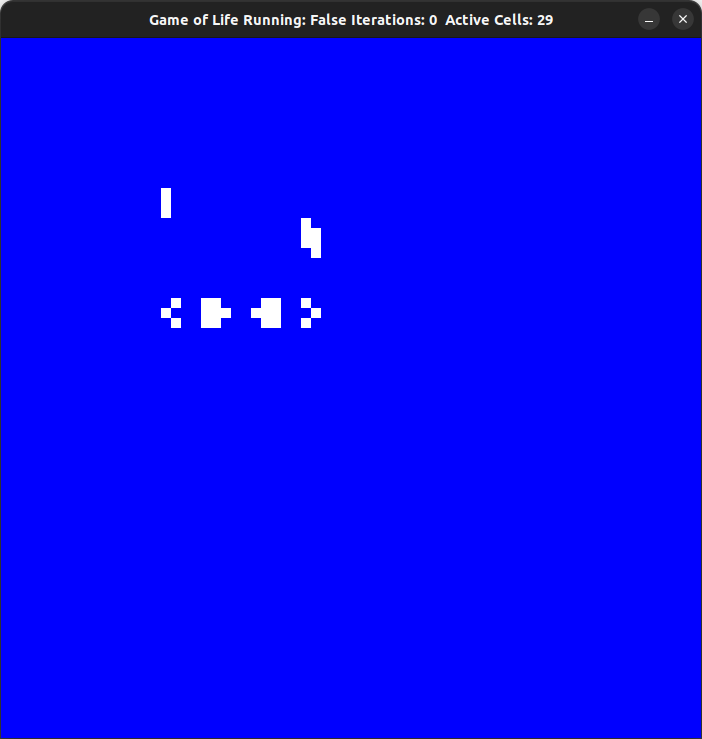
\includegraphics[width=0.5\textwidth]{osciladores.png}
            \end{figure}
            \subsubsection{Vidas estáticas}
            Son patrones que no cambian de una generación a la siguiente. Se consideran osciladores de periodo 1.
            \begin{figure}[h!]
                \centering
                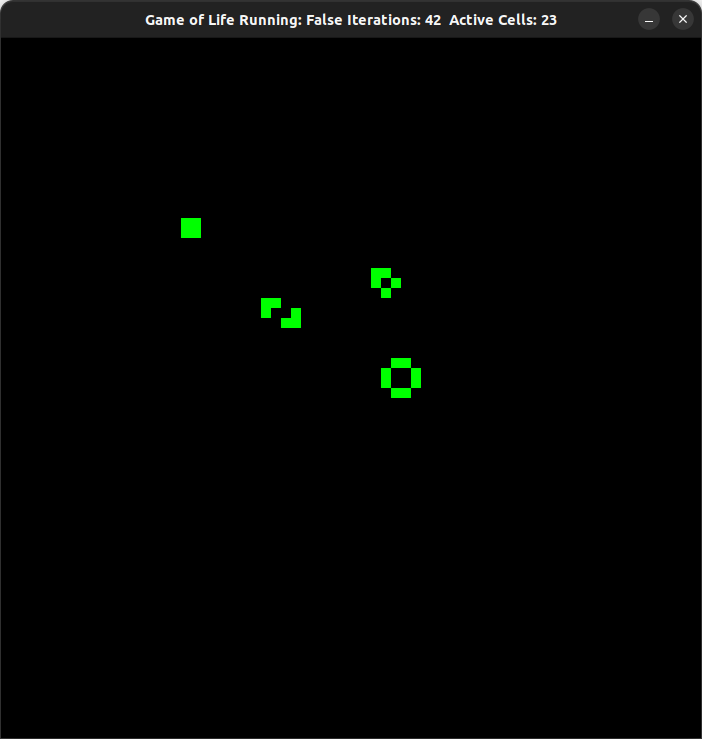
\includegraphics[width=0.5\textwidth]{fijas.png}
            \end{figure}
            \subsubsection{Planeadores}
            Son patrones que reqparecen en otra posición tras completar su periodo. Es decir, son patrones que tras un periodo fijo vuelven a su posicion original.
            \begin{figure}[h!]
                \centering
                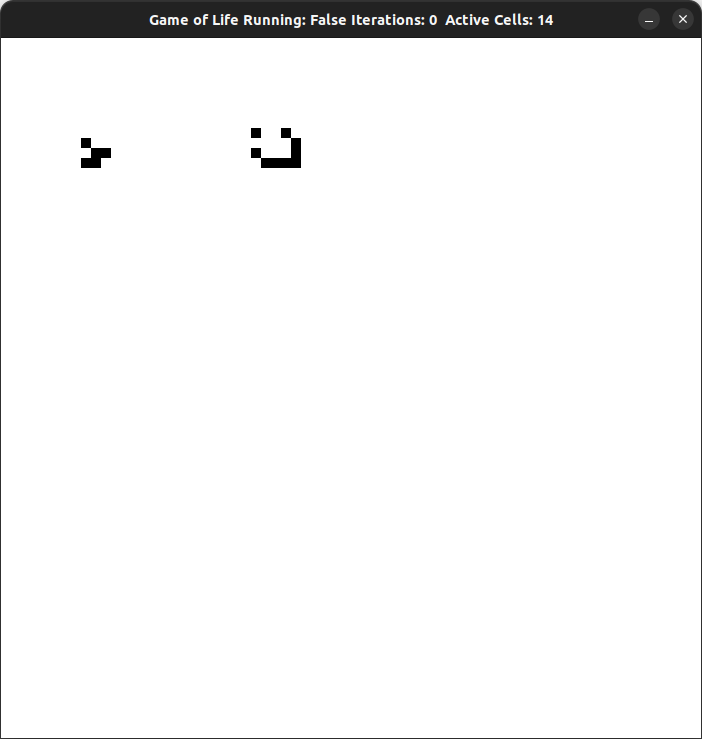
\includegraphics[width=0.5\textwidth]{planeadores.png}
            \end{figure}
            \subsubsection{Matusalenes}
            Son patrones que pueden evolucionar a lo largo de muchos turnos antes de estabilizarse. 
            \begin{figure}[h!]
                \centering
                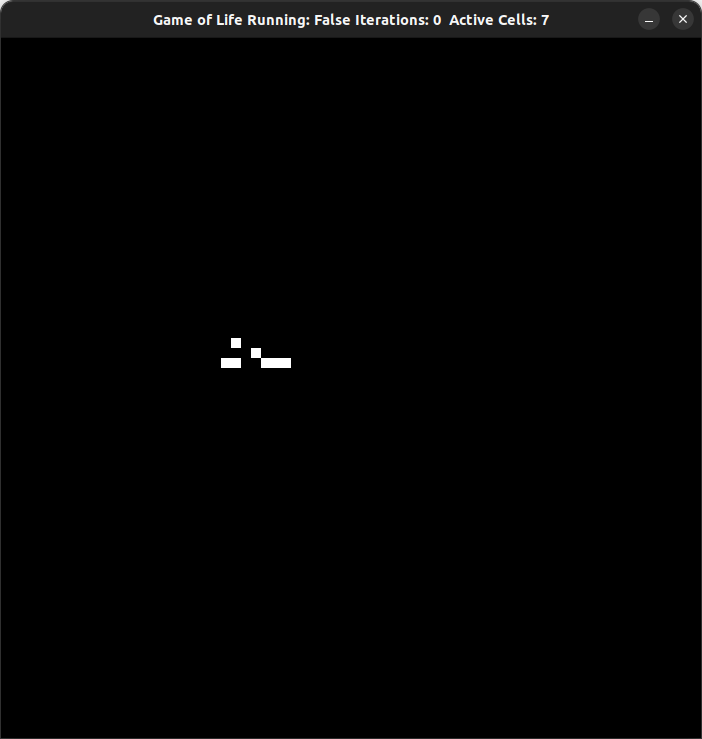
\includegraphics[width=0.5\textwidth]{matusalen.png}
            \end{figure}
            \subsection{Gráficas de densidad}
            También para cada "ronda" nueva se implementó una gráfica de densidad poblacional de células vivas respecto a el tamaño total de la población.
                \subsubsection{Ejemplo con un matusalén}
                \begin{figure}[h!]
                    \centering
                    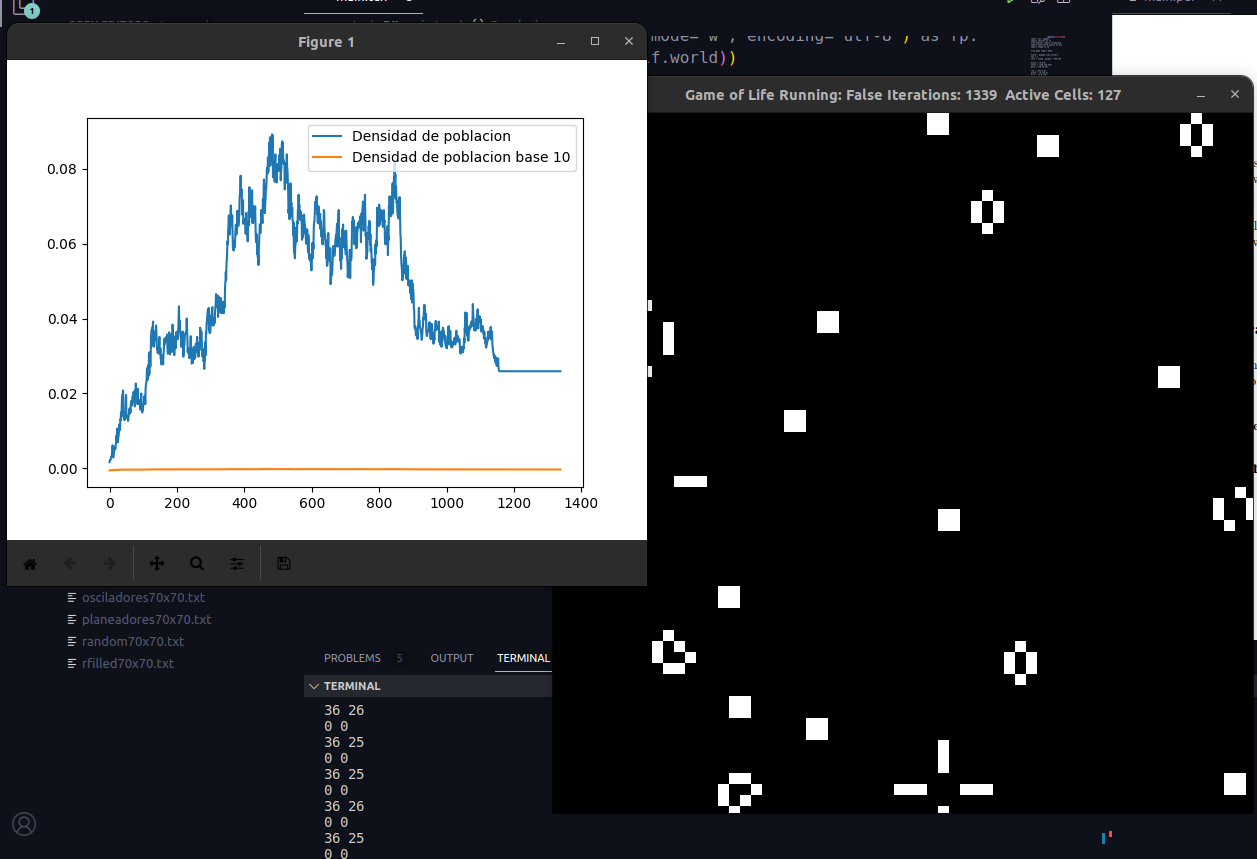
\includegraphics[width=0.6\textwidth]{grafica.png}
                \end{figure}
                \newpage
        \subsection{Código}
            El programa se basa en 2 archivos, el main, que se encarga de la ventana y eventos; y el archivo game.py que se encarga de la lógica del autómata.
            \subsubsection{main.py}
            \lstset{language=Python}
                \begin{lstlisting}
import sys, pygame
import tkinter as tk
from tkinter import filedialog
import matplotlib.pyplot as plt
import numpy as np

from game import Game

Clock = pygame.time.Clock()
fps = 1
size = width, height = 700,700

black = (0,0,0)
white = (255,255,255)
gray = (70,70,70)

red = (255,0,0)
green = (0,255,0)
blue = (0,0,255)
pink = (255,192,203)
colors = [white,black,gray,red,green,blue,pink]


def mouse_click(world: Game, mouse_x: int, mouse_y:int)->None:
    x = int(mouse_x/(world.get_cell_size) - (world.get_offset_x/world.get_cell_size))
    y = int(mouse_y/(world.get_cell_size) - (world.get_offset_y/world.get_cell_size))
    print(x,y)
    print(world.get_offset_x,world.get_offset_y)
    if world.get_cell_value(x,y) == world.live:
        world.set_cell_value(x,y,world.dead)
    else:
        world.set_cell_value(x,y,world.live)

def graph(b : list,s:int):
    s = np.array(s)
    population = np.divide(np.array(b),s)
    populationlog = np.divide(np.log10(population),s)
    plt.plot(population,label="Densidad de poblacion")
    plt.plot(populationlog, label="Densidad de poblacion base 10")
    plt.legend()
    plt.show()
    


def main():
    n,m = 0,0
    pygame.init()
    screen = pygame.display.set_mode(size)
    title = "Game of Life"
    pygame.display.set_caption(title)
    world = Game()
    
    if len(sys.argv) >1:
        print(sys.argv)
        n = int(sys.argv[1])
        m = int(sys.argv[2])
        color_live = int(sys.argv[3])
        color_dead = int(sys.argv[4])
        
        world.set_color(colors[color_live],colors[color_dead])
        world.set_size(n,m)
        world.__init__()
    running = False
    speed = 20
    zoom = 1
    plot_pop = []
    size_map = world.get_width * world.get_height
    while 1:
        for event in pygame.event.get():
            if event.type == pygame.QUIT:
                print("End")
                sys.exit()
            if event.type == pygame.MOUSEBUTTONDOWN:
                x, y = pygame.mouse.get_pos()
                mouse_click(world,x,y)
            if event.type == pygame.KEYDOWN:
                if event.key == pygame.K_RIGHT:
                    world.set_offset_x(world.get_offset_x+speed)
                if event.key == pygame.K_LEFT:
                    world.set_offset_x(world.get_offset_x-speed)
                if event.key == pygame.K_DOWN:
                    world.set_offset_y(world.get_offset_y+speed)
                if event.key == pygame.K_UP:
                    world.set_offset_y(world.get_offset_y-speed)
                if event.key == pygame.K_g and (not running):
                    graph(plot_pop,size_map)
                if event.key == pygame.K_SPACE:
                    running = not running
                if event.key == pygame.K_z:
                    world.set_cell_size(world.get_cell_size+zoom)
                if event.key == pygame.K_x:
                    world.set_cell_size(world.get_cell_size-zoom)
                if event.key == pygame.K_r:
                    world.init_map()
                    plot_pop = []
                if event.key == pygame.K_l:
                    file_path = filedialog.askopenfilename(filetypes=(
                        ("Text Files","*.txt"),
                        ("All Files", "*.*")
                    ))
                    print(file_path)
                    if file_path != "":
                        world.load_file(file_path)
                if event.key == pygame.K_s:
                    file_path = filedialog.asksaveasfilename(filetypes=(
                        ("Text Files","*.txt"),
                        ("All Files", "*.*")
                    ))
                    if file_path != "":
                        world.save_file(file_path)
        if running:
            world.update()
            plot_pop.append(world.get_live_cells)
            
        screen.fill((50,50,50))
        world.draw(screen)

        Clock.tick(60)
        pygame.display.set_caption(title+f" Running: {running} Iterations: {world.get_iterations}  Active Cells: {world.get_live_cells}")
        pygame.display.flip()



if __name__ == "__main__":
    main()
                \end{lstlisting}
		
        \subsubsection{game.py}
                \begin{lstlisting}
import pygame

class Game:
    width, height = 70,70    
    live = 1
    dead = 0

    color_live = (255,255,255)
    color_dead = (0,0,0)

    world = []
    new_world = []

    born = []
    alive = []

    cell_size = 10
    iterations = 0

    offset_x = 0
    offset_y = 0

    def __init__(self,pattern: str = "23/3"):
        self.init_map()
        self.alive = [int(v) for v in pattern.split("/")[0]]
        self.born = [int(v) for v in pattern.split("/")[1]]
    @property
    def get_height(self)->int:
        return self.height
    @property
    def get_width(self)->int:
        return self.width
    @property
    def get_iterations(self)->int:
        return self.iterations
    @property
    def get_live_cells(self)->int:
        return self.world.count(1)
    @property
    def get_cell_size(self)->int:
        return self.cell_size
    @property
    def get_offset_x(self)->int:
        return self.offset_x
    @property
    def get_offset_y(self)->int:
        return self.offset_y

    def set_size(self,a:int,b:int):
        self.width = a
        self.height = b
    def set_offset_y(self,value:int):
        self.offset_y = value
    def set_offset_x(self,value:int):
        self.offset_x = value
    def set_cell_size(self,value:int):
        self.cell_size = value
    def set_color(self,live:tuple,dead:tuple):
        self.color_live = live
        self.color_dead = dead

    def init_map(self):
        self.iterations = 0
        self.world = [0] * (self.width * self.height)
        self.new_world =  [0] * (self.width * self.height)
        self.offset_x = 0
        self.offset_y = 0

    def get_cell_value(self,x: int, y :int)->int:
        if x >= self.width:
            x -= self.width
        elif x < 0:
            x += self.width
        if y >= self.height:
            y -= self.height
        elif y < 0:
            y += self.height
        return self.world[(y * self.width) + x]
    def set_cell_value(self,x:int,y:int, value:int)->int:
        self.world[(y * self.width)+x] = value
    
    def update(self)->None:
        self.iterations += 1
        for y in range (self.height):
            for x in range (self.width):
                neighbors = [
                    self.get_cell_value(x + 1, y - 1),
                    self.get_cell_value(x , y - 1),
                    self.get_cell_value(x - 1, y - 1),
                    self.get_cell_value(x - 1, y),
                    self.get_cell_value(x + 1, y),
                    self.get_cell_value(x - 1, y + 1),
                    self.get_cell_value(x , y + 1),
                    self.get_cell_value(x + 1, y + 1),
                ]
                alive_count = neighbors.count(self.live)
                current = self.get_cell_value(x,y)
                if current == self.live:
                    if alive_count not in self.alive:
                        current = self.dead
                else:
                    if alive_count in self.born:
                        current = self.live
                self.new_world[(y * self.width) + x] = current

        for i in range (self.width * self.height):
            self.world[i] = self.new_world[i]

    def draw (self, context: pygame.Surface)->None:
        cell_size = self.cell_size
        ox = self.offset_x
        oy = self.offset_y
        for y in range (self.height):
            for x in range (self.width):
                current = self.get_cell_value(x,y)
                if current == self.live:
                    pygame.draw.rect(
                        surface=context,
                        color=self.color_live, 
                        rect=(x * cell_size + ox, y * cell_size  + oy , cell_size, cell_size))
                else:
                    pygame.draw.rect(
                        surface=context,
                        color=self.color_dead,
                        rect=(x * cell_size + ox, y * cell_size  + oy , cell_size, cell_size))
                        

    def save_file(self, filename: str = "state.txt")->None:
        with open(filename, mode="w", encoding="utf-8") as fp:
            fp.write(str(self.world))

    def load_file(self, filename: str = "state.txt")->None:
        with open(filename, mode="r", encoding="utf-8") as fp:
            data = fp.read()[1:-1]
            self.world = [int(v) for v in data.split(",")]
                \end{lstlisting}
    
    
    \section{Conclusiones}
    Hubieron muchas cosas interesantes en la realización de la práctica, empezando en la forma de abordar el problema. Uno pensaría que con matrices sería suficiente, pero la complejidad temporal y espacial se eleva mucho. Esta práctica demostró de manera excelente el comportamiento de los autómatas celulares. Ya que el juego de la vida puede tener diferentes variantes, se observaba también que al cambiar las restricciones, el comportamiento variaba mucho, siendo mas ordenado, o incluso más caótico. 
    \bibliographystyle{apacite}
    \begin{thebibliography}{1}
        \bibitem[1]{c0}Weisstein, E., 2021. Elementary Cellular Automaton. Recuperado 6 de noviembre de 2022, de \url{https://mathworld.wolfram.com/ElementaryCellularAutomaton.html}
        \bibitem[2]{c1} Caparrini, F. S. Autómatas Celulares - Fernando Sancho Caparrini. Recuperado 6 de noviembre de 2022, de \url{http://www.cs.us.es/%7Efsancho/?e=66}
        \bibitem[3]{c2} colaboradores de Wikipedia. (2022, 7 noviembre). Juego de la vida. Wikipedia, la enciclopedia libre \url{https://es.wikipedia.org/wiki/Juego_de_la_vida}
    \end{thebibliography}
    
\end{document}